\documentclass[JCDReport.tex]{subfiles} 
\begin{document}

\subsection{Code Coverage}

To measure the code coverage of the VFSBase and VFSBaseTests correctly, the DiskServiceReference has to be excluded from the coverage, because this code is generated automatically and therefore is irrelevant for the test coverage (WCF service reference). Figure \ref{fig:excludeTests} shows how this is done for the VFSBase project.\\

\begin{figure}[h!]
	\centering
	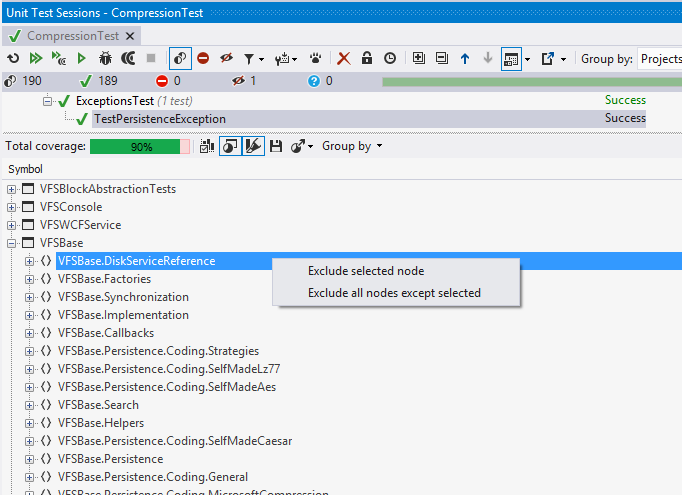
\includegraphics[scale=0.75]{Images/code_coverage1.png} 
	\caption{Exclude Tests}
	\label{fig:excludeTests}
\end{figure}	

The code coverage of the code was at 94\% on Monday, 2013-05-13 at 4.46 pm, see Figure \ref{fig:codeCoverage}.

\begin{figure}[h!]
	\centering
	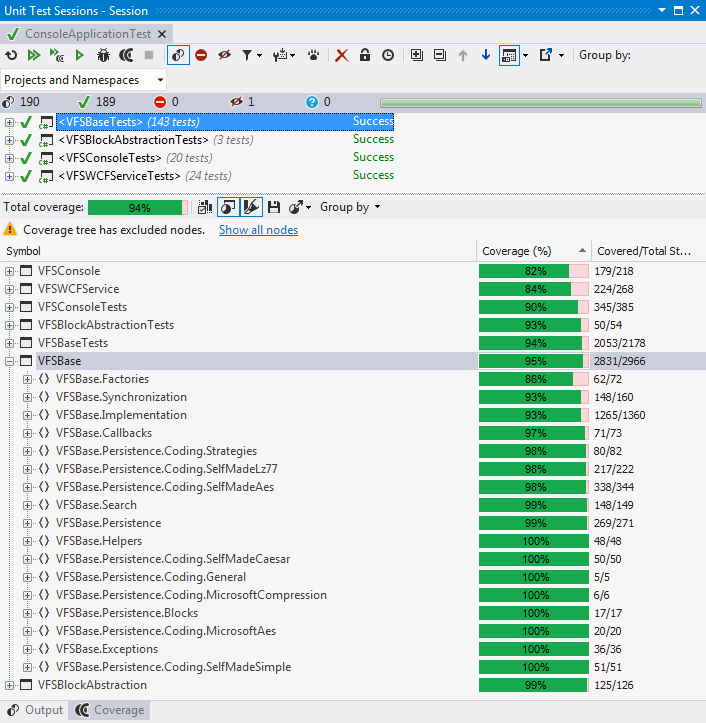
\includegraphics[scale=0.75]{Images/code_coverage.png} 
	\caption{Code Coverage}
	\label{fig:codeCoverage}
\end{figure}	

\subsection{Static Code Analysis}
The static code analysis was run with the JCD C\# ruleset. 
The Visual Studio didn't recognise that some methods in the view model are being used by the view in the xaml-files, which resulted in some warnings in the analysis, which were suppressed in the suppression file or directly in the code. Beside this few warnings there were none.

\end{document}